%Set document class
\documentclass{report}

%Load math symbol packages
\usepackage{amsmath}
\usepackage{amssymb}
\usepackage{graphicx}

%New commands
\newcommand{\solution}{\textbf{Solution: }}
\newcommand{\inner}[2]{\langle #1, #2 \rangle}

%Declare beginning of document
\begin{document}

%Center to make a document title
\begin{center}
	\huge{\bf Math 31BH: Assignment 3} \\
	Due 01/23 at 23:59 \\
	Merrick Qiu
\end{center}

\bigskip

%Start a numbered list (there are other list formats, such as itemize and description}
\begin{enumerate}

	\item
	Prove that the function $f \colon \mathbb{R} \to \mathbb{R}$ defined by $f(t)=|t|$ is continuous but 
	not differentiable at $t=0$.
	
	\solution 
	Since 
	\[
		\lim_{t\to0^-} \|t\| = \lim_{t\to0^+} \|t\| = \|0\| = 0
	\]
	$f(t)$ is continuous at $t=0$.
	
	The left hand limit for the derivative is
	\[
		\lim_{h\to0^-} \frac{f(0+h) + f(h)}{h} = \frac{2|h|}{h} = -1
	\]
	and the right hand limit for the derivative is
	\[
		\lim_{h\to0^+} \frac{f(0+h) + f(h)}{h} = \frac{2|h|}{h} = 1
	\]
	Since the left and right hand limits do not agree, 
	the function is not differentiable at $t=0$.

	\medskip
	\item
	Consider the differentiable function $g \colon \mathbb{R} \to \mathbb{R}^2$ given by
	$g(t)=(t,t^3)$.
	
		\begin{enumerate}
		
			\smallskip
			\item
			Sketch the tangent vector and the tangent line at $t=0$ and $t=1.$
			
			\smallskip
			\item
			Construct a function $h \colon \mathbb{R} \to \mathbb{R}$ with the 
			same image as $g$ such that $g(0)=h(0)$ but $h$ is not differentiable
			at $t=0$.
		
		\end{enumerate}			
		
	\solution

	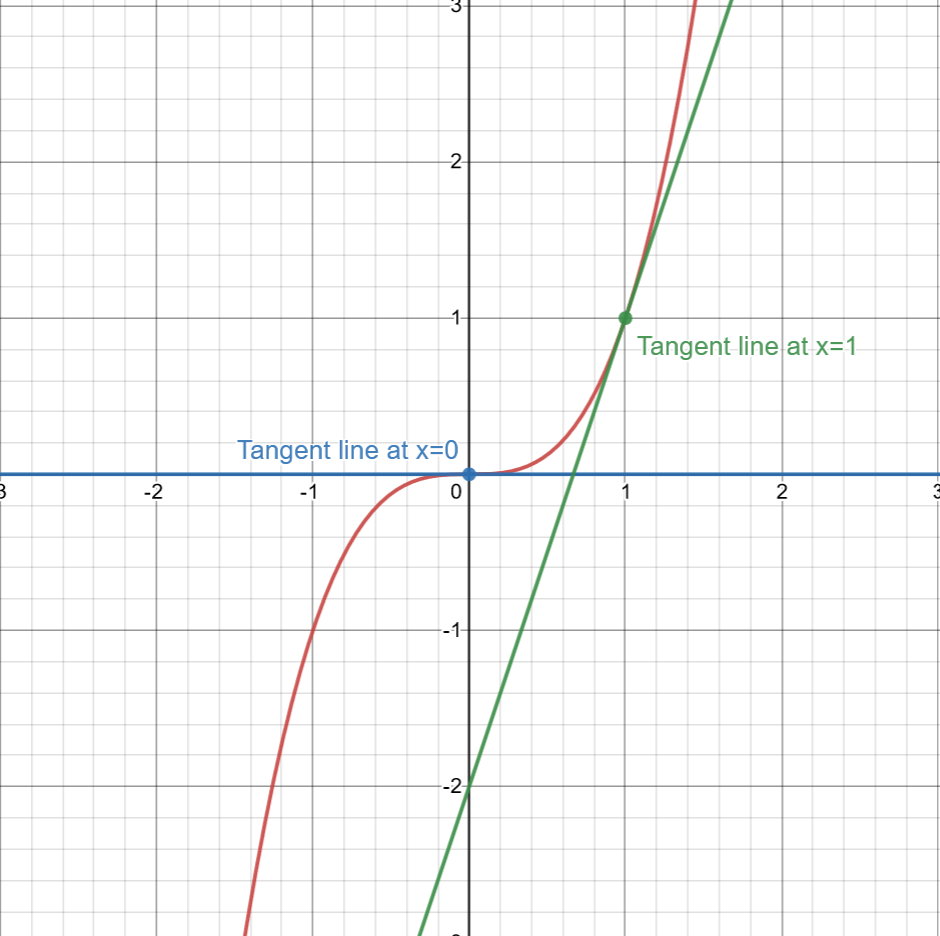
\includegraphics[scale=0.5]{Problem2a.png} 

	The function $h(t) = (t^{\frac{1}{3}}, t)$ has the same image as $g$
	but it is not differentiable at $t=0$ because the derivative of
	$t^{\frac{1}{3}}$, which is $\frac{1}{3}t^{-\frac{2}{3}}$,
	is undefined at $t=0$.

	\medskip
	\item
	Consider the differentiable function $f \colon \mathbb{R} \to \mathbb{R}^2$ defined by
	$f(t) = (e^{kt}\cos t, e^{kt} \sin t)$ where $k$ is a constant.
	
		\begin{enumerate}
		
			\smallskip
			\item
			Sketch the image of $f$.
			
			\smallskip
			\item
			Prove that
			
				\begin{equation*}
					\frac{f'(t) \cdot f(t)}{\|f'(t)\| \| f(t)\|} = \frac{k}{\sqrt{1+k^2}}.
				\end{equation*}
				
			\smallskip
			\item
			Prove that the angle between the tangent vector $f'(t)$ and the line 
			joining $f(t)$ to $(0,0)$ is the same for all $t \in \mathbb{R}$.
		
		\end{enumerate}
		
	\solution 

	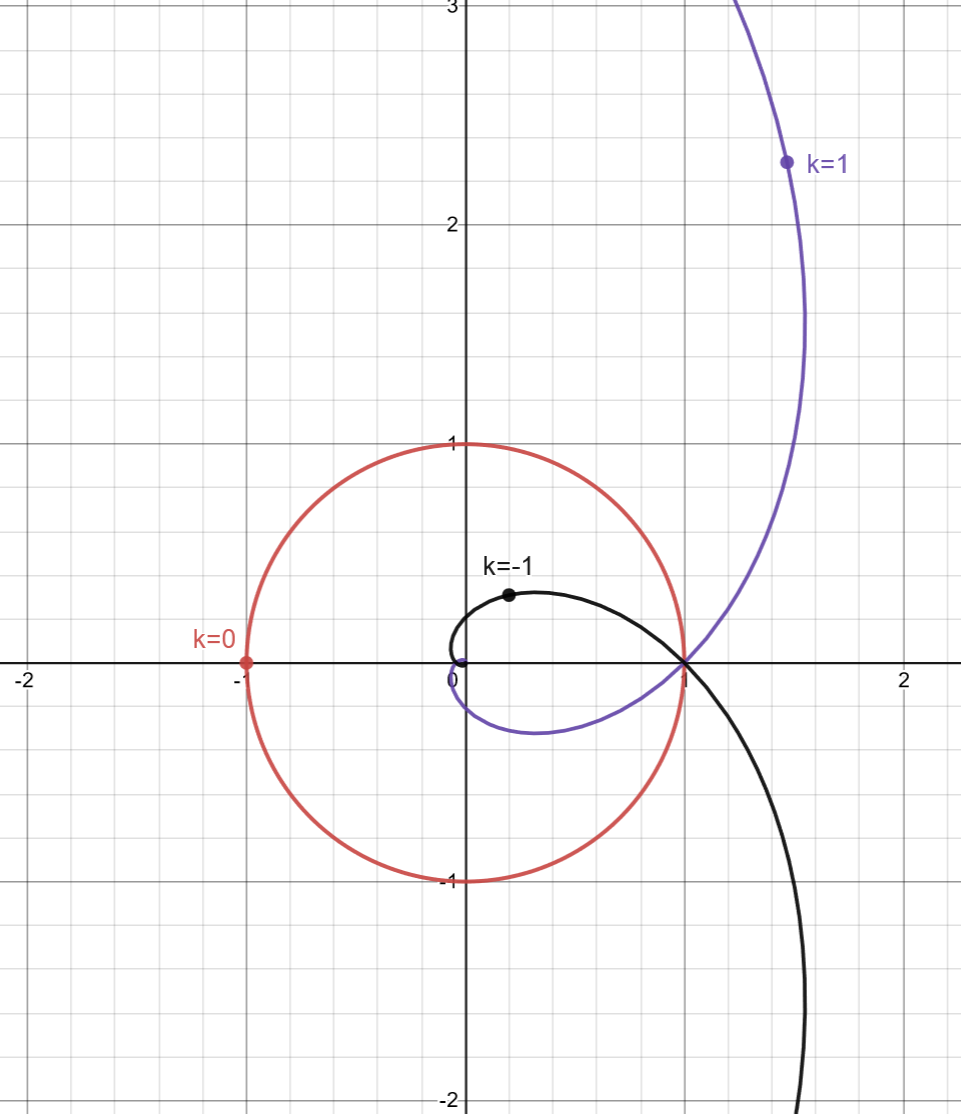
\includegraphics[scale=0.5]{Problem3a.png} 

	The derivative of $f$ is 
	$f'(t) = (ke^{kt}\cos(t)-e^{kt}\sin(t), ke^{kt}\sin(t)+e^{kt}\cos(t))$ so 
	\begin{align*}
		f'(t)\cdot f(t) 
		&= e^{kt}\cos(t)(ke^{kt}\cos(t)-e^{kt}\sin(t)) +
		   e^{kt}\sin(t)(ke^{kt}\sin(t)+e^{kt}\cos(t)) \\
		&= ke^{2kt}\cos^2(t) - e^{2kt}\sin(t)\cos(t) +
		   ke^{2kt}\sin^2(t) + e^{2kt}\sin(t)\cos(t) \\
		&= ke^{2kt}(\cos^2(t)+\sin^2(t)) + 
		   (e^{2kt}\sin(t)\cos(t)-e^{2kt}\sin(t)\cos(t)) \\
		&= ke^{2kt}
	\end{align*}
	The norm of $f(t)$ is 
	\[
		\|f(t)\| =
		\sqrt{e^{2kt}\cos^2(t) + e^{2kt}\sin^2(t)} =
		\sqrt{e^{2kt}(\cos^2(t) + \sin^2(t))} =
		e^{kt}
	\]
	and the norm of $f'(t)$ is 
	\begin{align*}
		&\|f'(t)\| 
		= \sqrt{(ke^{kt}\cos(t)-e^{kt}\sin(t))^2 + 
			(ke^{kt}\sin(t)+e^{kt}\cos(t))^2} \\
		&= \sqrt{k^2e^{2kt}\cos^2(t)-2ke^{2kt}\sin(t)\cos(t)+e^{2kt}\sin^2(t) + 
			k^2e^{2kt}\sin^2(t)+2ke^{2kt}\sin(t)\cos(t) +e^{2kt}\cos^2(t)} \\
		&= \sqrt{k^2e^{2kt} + e^{2kt}} \\ 
		&= e^{kt}\sqrt{k+1}
	\end{align*}

	Therefore, 
	\[
		\frac{f'(t)\cdot f(t)}{\|f'(t)\|\|f(t)\|} =
		\frac{ke^{2kt}}{e^{2kt}\sqrt{k+1}} =
		\frac{k}{\sqrt{1+k}}
	\]

	Since $\cos(\theta) = \frac{v\cdot w}{\|v\|\|w\|}$ for any two vectors $v, w$,
	the equation from part b states that the cosine between 
	$f(t)$ and $f'(t)$ is constant for all values of $t$.
	Therefore, the angle between the tangent vector and the line joining 
	$f(t)$ to the origin is the same for all $t \in \mathbb{R}$.
\end{enumerate}
%Declare end of document
\end{document}